\def\nodeA{node [anchor=east] {$S_1$}}
\def\nodeB{node [anchor=west] {$S_2$}}
\def\nodeT{node [left=0.4cm] {\tiny $T_1$} node [right=0.4cm] {\tiny $T_2$}}
% Definition of circles
\def\firstcircle{(0,0) circle (1.5cm)}
\def\secondcircle{(0:2cm) circle (1.5cm)}
\def\thirdcircle{(0:1cm) circle (1.11cm)}

\colorlet{circle edge}{blue!50}
\colorlet{circle area}{blue!20}

\tikzset{filled/.style={fill=circle area, draw=circle edge, thick,color=lightgray},
    outline/.style={draw=circle edge, thick}}


% Set  A impossible B
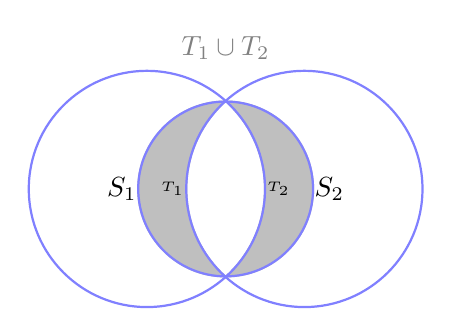
\begin{tikzpicture}
    \begin{scope}
        \clip \firstcircle;
        \draw[filled, even odd rule] \secondcircle
                                     \thirdcircle;
    \end{scope}
    \begin{scope}
        \clip \secondcircle;
        \draw[filled, even odd rule] \firstcircle
                                     \thirdcircle;
    \end{scope}

    \draw[outline] \firstcircle \nodeA;
    \draw[outline] \secondcircle \nodeB;
    \draw[outline] \thirdcircle \nodeT;
    \node[anchor=south] at (current bounding box.north) {\color{gray}$T_1 \cup T_2$};
\end{tikzpicture}